\section{Diagrama de Implantação}
\label{sec:titSecDiagDeploy}

O Diagrama de Implantação \cite[determina as necessidades de \textit{hardware} do sistema, as características físicas como servidores, estações, topologias e protocolos de comunicação]{guedes2018uml}, destacando todos as necessidades físicas no qual o sistema deverá ser executado. Também é mostrado como será a distribuição dos módulos do sistema nos momentos onde a aplicação estará sendo executada em diferentes servidores.

\begin{figure}[H]
    \centering
    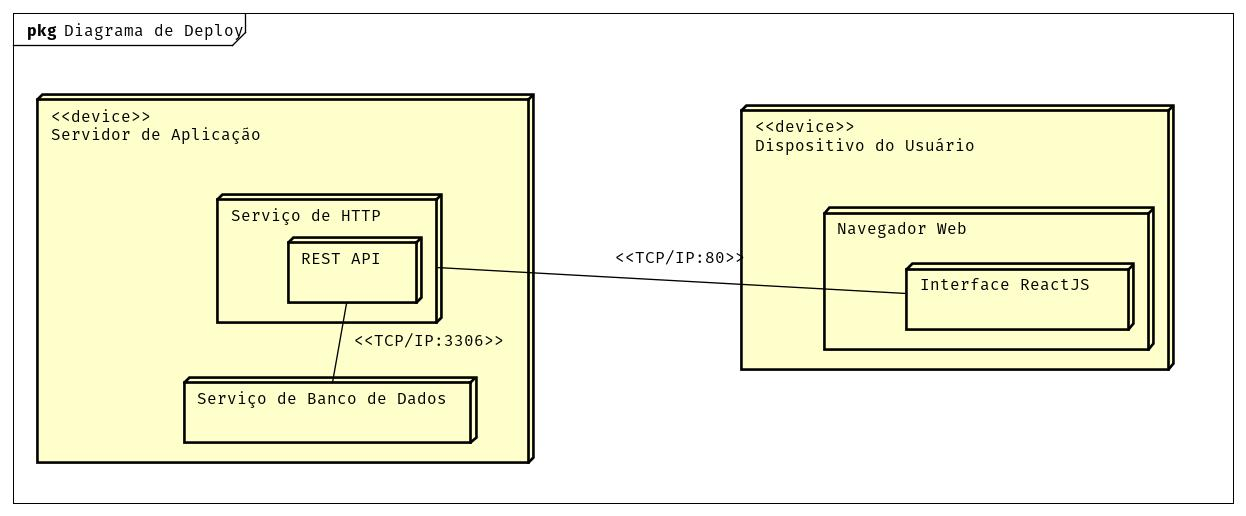
\includegraphics[width=13cm]{./dados/analise/diagramadeploy.jpg}
    \caption{Representação do Diagrama de Implantação do Sistema}
    \label{fig:diagramaDeploy}
\end{figure}

A \autoref{fig:diagramaDeploy} mostra a aplicação desse conceito no projeto em questão. Nela é possível observar a distribuição do sistema em dois nós principais. O primeiro é o servidor de aplicação, que ecapsula o servidor Apache. Nesse mesmo servidor é possível observar a presença de um servidor de banco de dados MySQL, o qual será responsável por armazenar os dados do sistema.
O outro nó, representa o lado do cliente da aplicação, responsável pelas chamadas aos \textit{endpoints} da API Rest contida no servidor \textit{web}.
